% So You Want To Be a Computational Biologist
%
% A brief introduction to emphasise that bioinformatics is biology,
% even if a particular skill set, and that acquiring that skill set will
% need practice.

\subsection{So You Want To Be a Computational Biologist?}
\begin{frame}
  \frametitle{What is this ``bioinformatics'' thing, anyway?}
  \begin{itemize}
    \item Bioinformatics: biology using computational and mathematical tools
    \item A discipline within biology
    \begin{itemize}
      \item Loman \& Watson (2013) ``So you want to be a computational biologist?''
        \url{http://dx.doi.org/10.1038/nbt.2740}
      \item Welch \textit{et al.} (2014) ``Bioinformatics Curriculum Guidelines: Toward a Definition of Core Competencies''
      \url{http://dx.doi.org/10.1371/journal.pcbi.1003496}
      % http://bit.ly/1fS4iDJ links to http://biomickwatson.wordpress.com/2014/03/10/the-only-core-competency-youre-ever-going-to-need/}
      \item Watson (2014) ``The only core competency you need'' \url{http://bit.ly/1fS4iDJ} (blog)
    \end{itemize}
  \end{itemize}
\end{frame}

\subsection{So You Want To Be a Computational Biologist?}
\begin{frame}
  \frametitle{What is this ``bioinformatics'' thing, anyway?}
  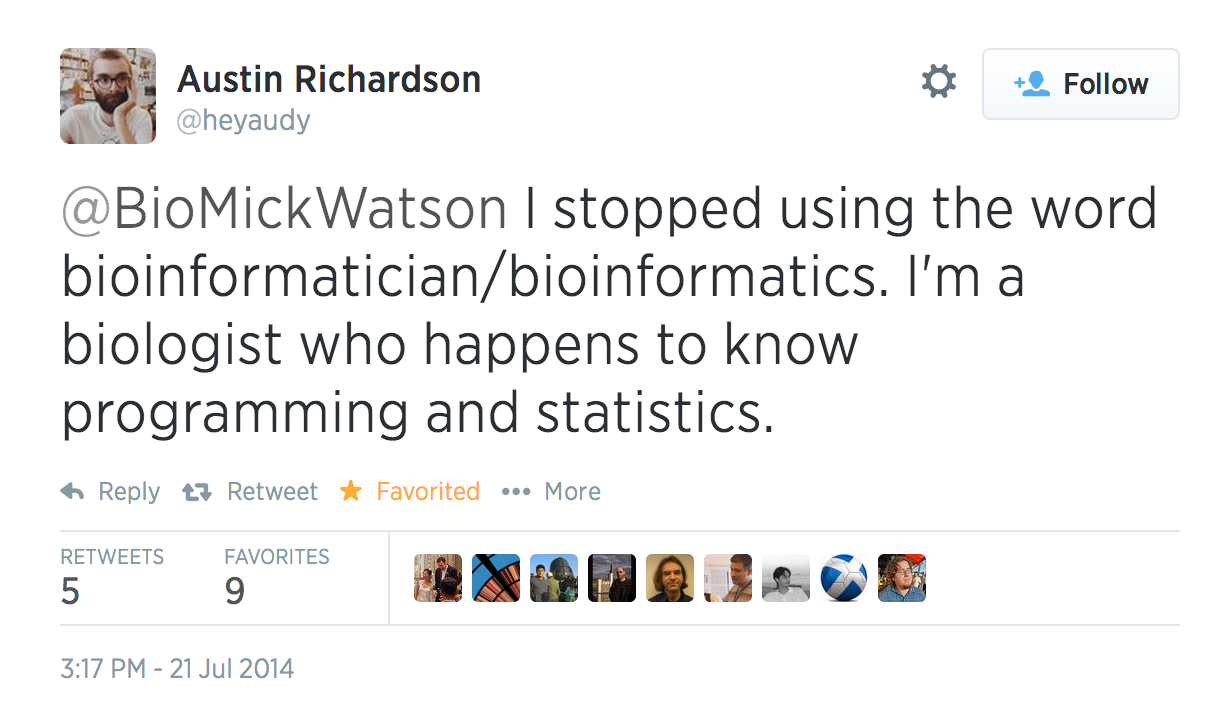
\includegraphics[width=.5\textwidth]{images/twitter_bioinformatician}
  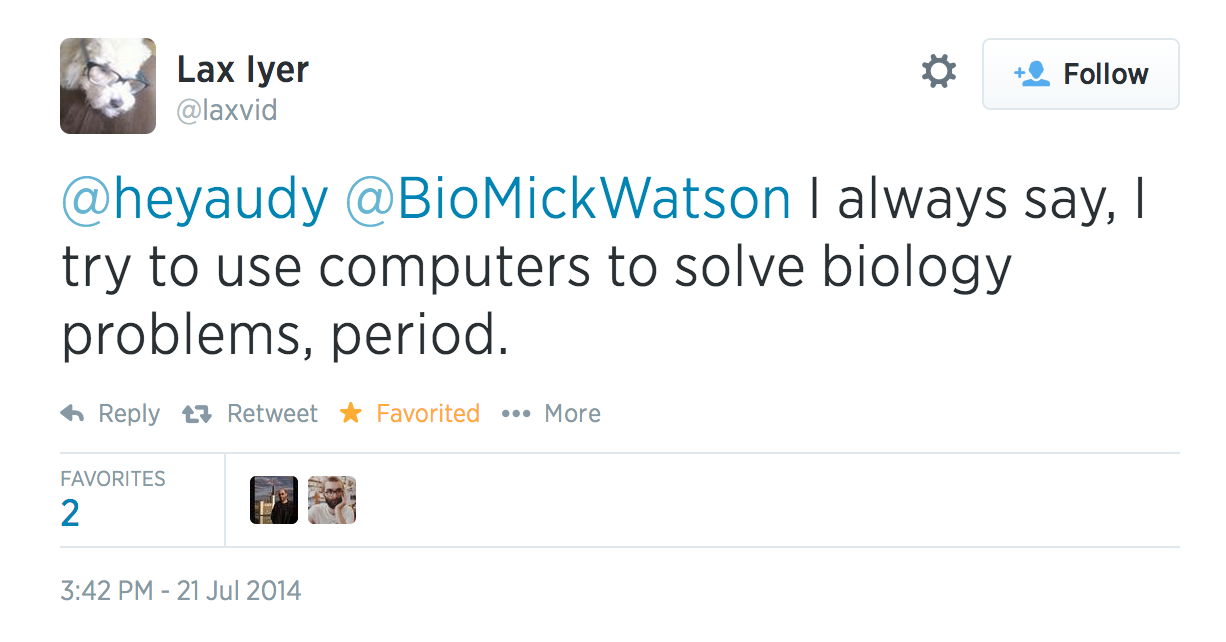
\includegraphics[width=.5\textwidth]{images/twitter_computers_biology}  
\end{frame}

\subsection{So You Want To Be a Computational Biologist?}
\begin{frame}
  \frametitle{Some uncomfortable truths}
  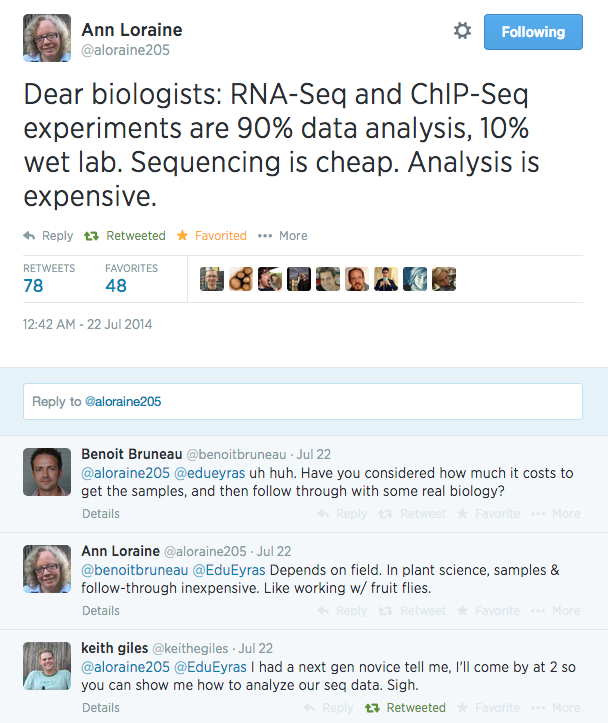
\includegraphics[width=.5\textwidth]{images/twitter_rnaseq}
  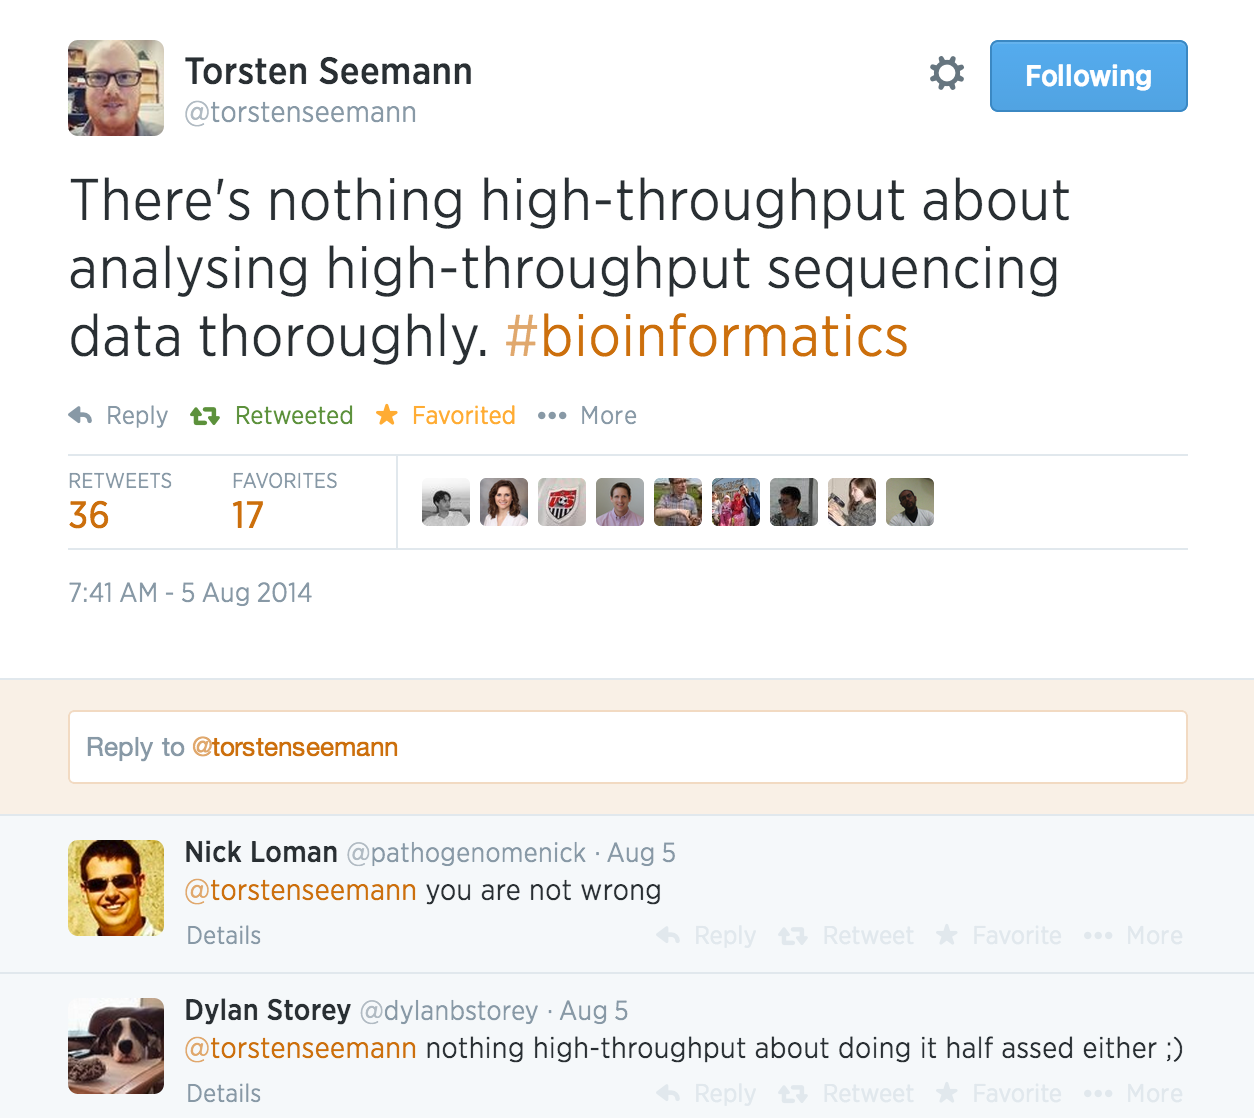
\includegraphics[width=.5\textwidth]{images/twitter_high_throughput}  
\end{frame}

\begin{frame}
  \frametitle{Some uncomfortable truths}
  \begin{itemize}
    \item<1-> This one-day course will not make you a bioinformatician
    \begin{itemize}
      \item<2-> But practice might$\ldots$
    \end{itemize}
    \item<3-> The best way to learn is to do (``I don't know how to do this \emph{yet}, but I will find out.'')
    % http://bit.ly/Rq0D61 links to http://biomickwatson.wordpress.com/2013/08/06/bioinformatics-is-not-something-you-are-taught-its-a-way-of-life/
    \begin{itemize}
      \item \url{http://bit.ly/Rq0D61} (``Bioinformatics is a way of life'')
    \end{itemize}
    \item<3-> Most bioinformatics is problem-solving
    \item<3-> We will introduce some useful tools and concepts
  \end{itemize}
\end{frame}

\begin{frame}
  \frametitle{What it takes to be a bioinformatician}
  \begin{columns}[t]
    \begin{column}{5cm}
      \begin{itemize}
        \item Patience (problem-solving)
        \item Suspicion (statistics)
        \item Biological knowledge
        \item Social skills (no-one knows everything: ask!)
        \item Lots of practice          
      \end{itemize}
    \end{column}
    \begin{column}{5cm}
      \begin{itemize}
        \item Self-confidence (challenge results and dogma)
        \item Core domain skills: biology, computer science, statistics
        \item Deliver results (qualified, honest)
      \end{itemize}
    \end{column}
  \end{columns}
  \begin{itemize}
  % http://bit.ly/1jDuQsO link goes to http://biomickwatson.wordpress.com/2013/03/18/the-alternative-what-it-takes-to-be-a-bioinformatician/
    \item Watson (2014) ``What it takes to be a bioinformatician'' \url{http://bit.ly/1jDuQsO} (blog)
    %\item \url{http://science.slashdot.org/comments.pl?sid=3161217&cid=41542125}
  \end{itemize}
\end{frame}

\begin{frame}
  \frametitle{More general advice?}
  \begin{itemize}
    \item Ask us (we do this a lot)
    \item BioStars (\url{https://www.biostars.org})
    \item SeqAnswers (\url{http://seqanswers.com/})
    \item \textit{PLoS Comp Biol} collections (\url{http://www.ploscollections.org/static/pcbiCollections})
 \end{itemize}
 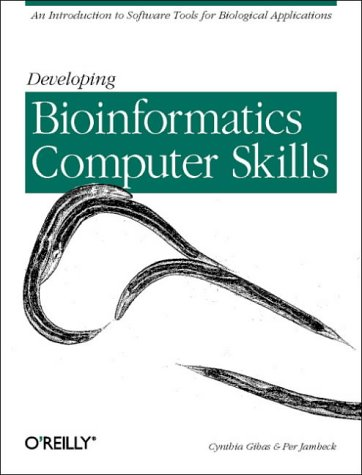
\includegraphics[width=.2\textwidth]{images/gibas_book}
 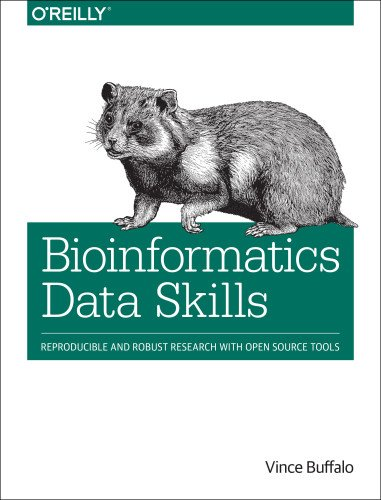
\includegraphics[width=.2\textwidth]{images/buffalo_book}
 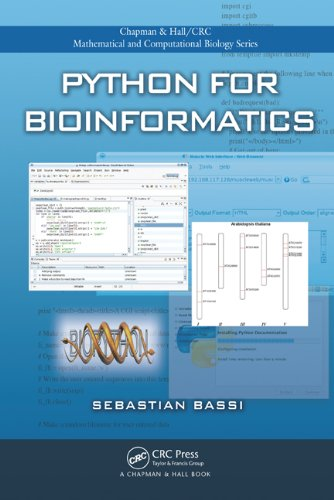
\includegraphics[width=.18\textwidth]{images/bassi_book}
 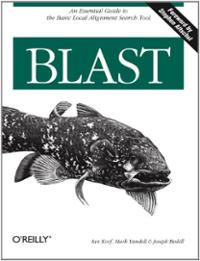
\includegraphics[width=.2\textwidth]{images/korf_book}
 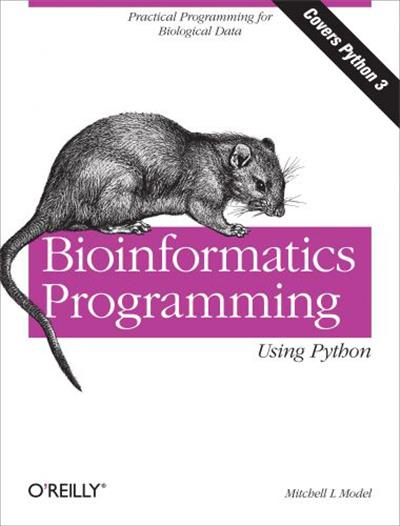
\includegraphics[width=.2\textwidth]{images/model_book}
\end{frame}
